\chapter{User manual for the 2 GW model}

 \begin{table}[H]
 \centering
\begin{tabular}{|c|c|}
\hline
\textbf{$I_{D\_ref}$ control} & \textbf{Power through MMC-2} \\ \hline
0                    & 0 MW                         \\ \hline
0.2                  & 475 MW                       \\ \hline
0.4                  & 950 MW                       \\ \hline
\end{tabular}
\caption{Power flow control in MMC-2}
\label{tab:Power_flow_control_in_MMC-2}
\end{table}


\section{Core assignment in RSCAD}
\begin{figure}[H]
\begin{subfigure}{.5\textwidth}
  \centering
  % include first image
  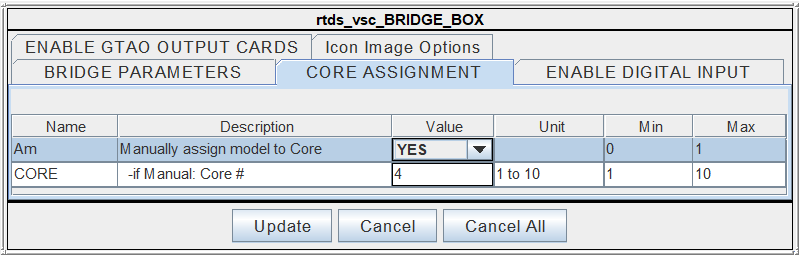
\includegraphics[height = 3cm,width = 8cm]{Diagrams/Chapter_4/Core_assignment_OWF1.PNG}  
  \caption{Core assignment of OWF-1}
  \label{fig:Core_assignment_OWF1}
\end{subfigure}
\begin{subfigure}{.5\textwidth}
  \centering
  % include second image
  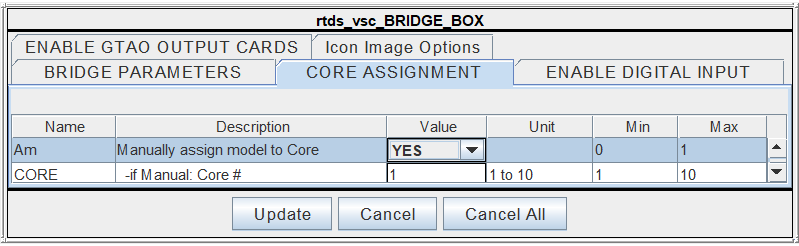
\includegraphics[height = 3cm,width = 8cm]{Diagrams/Chapter_4/Core_assignment_OWF2.PNG}  
  \caption{Core assignment of OWF-2}
  \label{fig:Core_assignment_OWF2}
\end{subfigure}

\newline

\begin{subfigure}{.5\textwidth}
  \centering
  % include third image
  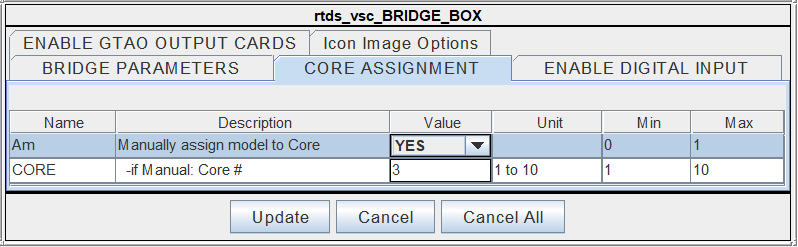
\includegraphics[height = 3cm,width = 8cm]{Diagrams/Chapter_4/Core_assignment_OWF3.PNG}  
  \caption{Core assignment of OWF-3}
  \label{fig:Core_assignment_OWF3}
\end{subfigure}
\begin{subfigure}{.5\textwidth}
  \centering
  % include fourth image
  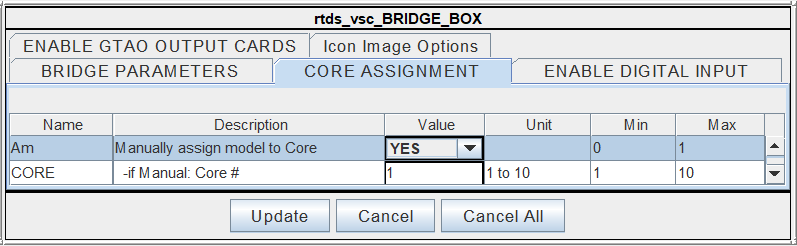
\includegraphics[height = 3cm,width = 8cm]{Diagrams/Chapter_4/Core_assignment_OWF4.PNG}  
  \caption{Core assignment of OWF-4}
  \label{fig:Core_assignment_OWF4}
\end{subfigure}
\caption{Core assignment of the 4 small time-step boxes representing 4 OWFs}
\label{fig:Complete_Core_assignment_OWF}
\end{figure}

After assigning the cores for the small-time step blocks, the processor assignment for subsystem 2 is as illustrated in Figure \ref{fig:subsystem2_processor}.

\begin{figure}[H]
\centering
%\hspace*{-2.2cm}
    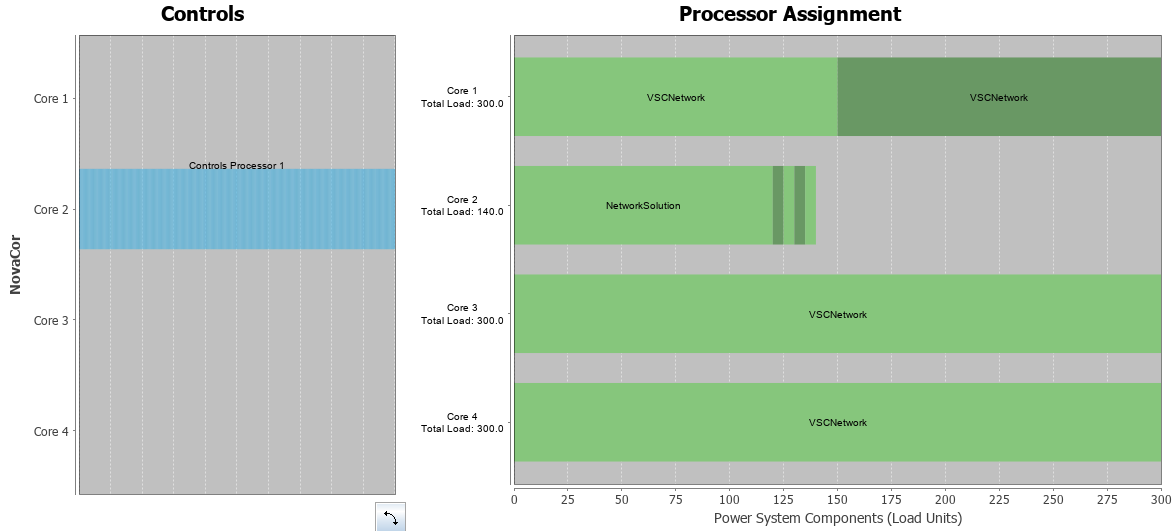
\includegraphics[height = 8cm,width = 17cm]{Diagrams/Chapter_4/subsystem2_processor.PNG}
    \caption{Processor assignment chart for subsystem 2}
    \label{fig:subsystem2_processor}
\end{figure}

The 'Core Assignment' tab is available by right-clicking the small-time block and choosing "Edit" and then "Parameters" as shown in Figure \ref{fig:Complete_Core_assignment_OWF}. Setting the 'Am' parameter to 'No' for all the small-time blocks causes all the available cores to be full and leaving no room for a processor to allocate control signals. Hence these cores should be manually assigned, and proper allocation has to be done.


\section{Configuring Tline module}\label{config_Tline}
The parameters are entered in the Tline popup menu and the file is compiled and saved in a ".clo" format.

The cable parameters are referenced through the external file previously created using the cable module. %Initially, a Bergeron cable model is created with RLC parameters in the Tline module. 
The ".clo" file must be added first using the 'Dnm1' option, which is obtained by double-clicking on the calculation box (Figure \ref{fig:Tline_calculationbox_RSCAD}). The cable constants are of type Bergeron as chosen in the 'cntyp' parameter in Figure \ref{fig:CableConfig}.

\begin{figure}
  \centering
  % include second image
  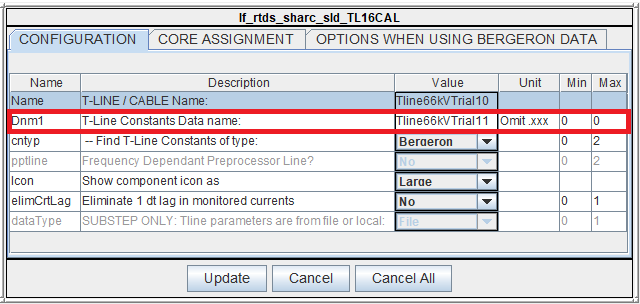
\includegraphics[height = 4cm,width = 9cm]{Diagrams/Chapter_4/TlineParaBlock_side1_mark.png}  
  \caption{Configuring Tline model in RSCAD}
  \label{fig:Tline_config_RSCAD}
\end{figure}